\documentclass[../main.tex]{subfiles}

\begin{document}
\pagebreak
\section{Description}
In this section, we will give a description of our overall system as well as a justification for our system and diagrams to support the description of the overall system.

	\subsection{Focus on properties}\label{sec: properties}
	Our system contains a lot of properties, to make all of these properties clear we use an enumeration.
	\begin{enumerate}
		\item The user can see the connection status to the server on the top right of the home screen. The user can also create a party from here and go to the settings and join a party screen.
		\item If the user's phone is disconnected to the server, then the player cannot use the create and join party buttons.
		\item Our application has a few settings: the user can change and save their name. This name will be shown in the lobby. The user can toggle btween offline/online mode using a button and the user can tobble between muted and unmuted music (heard in-game) using a button.
		\item The user can join a party by filling in the game pin of that party and clicking on enter.
		\item The user can select abilities in the lobby. The user can select three abilities which will be displayed in the game in the order they are chosen. The user can also see the master of the party, all the other party members, the ready status of the other party members and the party's game pin.
		\item If the user is the master of their party, they can start the game by pressing the button, provided all other players are ready. If the user is not the master of their party they can get (un)ready by pressing the button.
		\item The user can see the health of their character in the top right corner when in-game. This value changes in real-time when the character takes damage or is healed.
		\item When playing with multiple players, every player has a differently colored character.		
		\item While in-game, the user can walk around using the joystick and activate abilities, when they are not on a cooldown (they will appear opaque when on cooldown), using the corresponding buttons on the bottom right. 
		\item The abilities have various effects, but in our current implementation the user can teleport 4 tiles in the direction the character is facing, the user can damage other entities using arrows and a melee attack and the user can heal itself with ten health.
		\item When a player's health is displayed in the upper right corner when in-game. When it drops to zero, the player respawns at the level's spawnpoint.		
		\item The enemies fight back using their well developed A.I.
		\item When the boss is defeated, the player(s) return(s) to the lobby.
\end{enumerate}

\noindent
Here are some screenshots of our app, that give am idea of how the app looks and which activities we mean when talking about them. 		
		\begin{figure}[H]
			\centering
			\begin{minipage}{.45\textwidth}
				\centering
				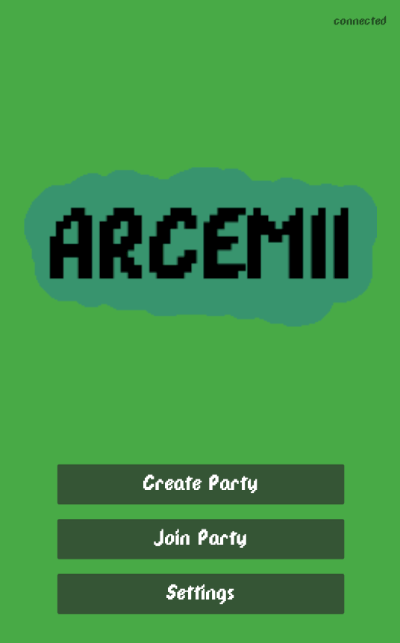
\includegraphics[width=\textwidth]{screenshots/main.png}
			\end{minipage}
			\begin{minipage}{.45\textwidth}
				\centering
				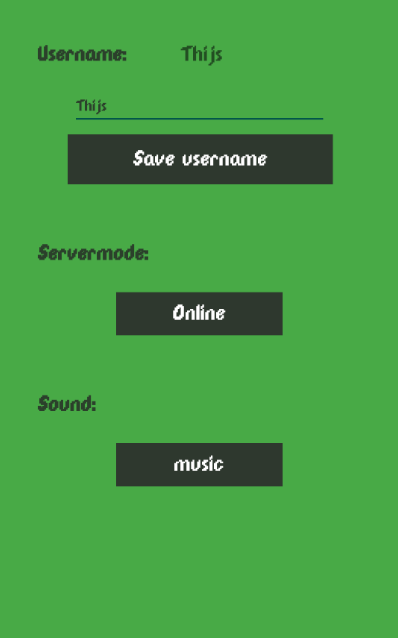
\includegraphics[width=\textwidth]{screenshots/settings.png}
			\end{minipage}
			\caption{The main-menu and the settings menu of the app. The homescreen features an animated gif.}
		\end{figure}
		
		\begin{figure}[H]
    	\centering
    	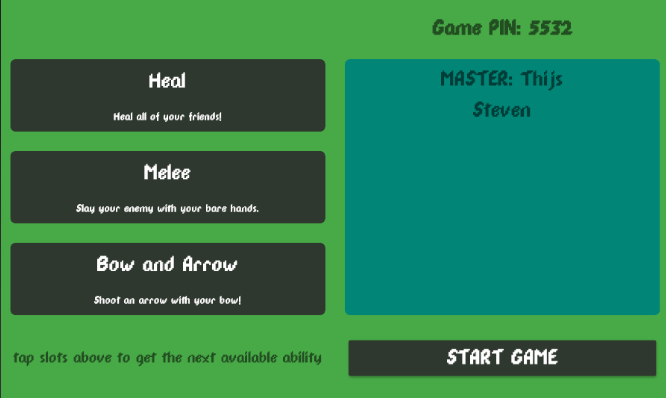
\includegraphics[width=.8\textwidth]{screenshots/party.png}
			\caption{The lobby of the app. On the left you can choose your abilities, on the right you can see the members of the party. If members press ready, `ís ready' appears after their name.}
  	\end{figure}
		\begin{figure}[H]
    	\centering
			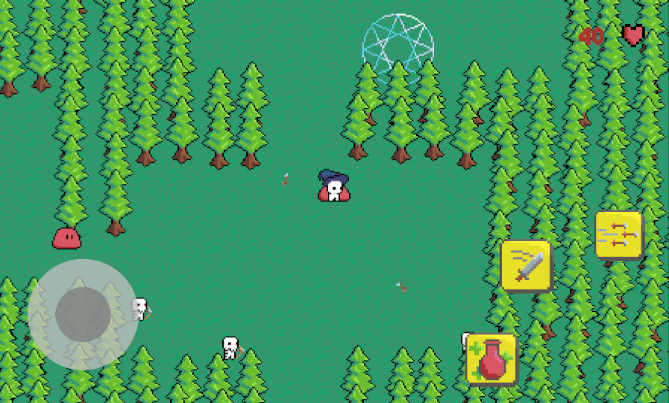
\includegraphics[width=.8\textwidth]{screenshots/game.png}
			\caption{The actual game. You are the player in the center of the screen. On the bottom right you can see two skeletons shooting arrows. On the left and behind the player, you can see a slime. Other players (not visible here) have a differently colored hat. Your health points are shown in the upper right corner.}
  	\end{figure}
    
	\subsection{Product justification}
	Our game can be categorised as a roguelike. A roguelike is a genre characterized by a dungeon crawl through procedurally generated levels with permanent death. We added some new flavours to it, like the ability to play it with more than one player. This is not normal for a roguelike, but we think it’s an interesting design choice. We really wanted to focus on the multiplayer aspect of the game, that’s why you select everything you need inside the lobby. If we would have done this inside the game, we would have created an unnecessary delay inside the game itself. You can also strategize with your friends before the game starts inside the lobby. We wanted a game that can be played in a short amount of time, like when you have a break for example. That’s why you also clear one floor per game. 
	
Most roguelikes are also tile-based and have a turn-based gameflow, this is also the reason why it’s hard to implement multiplayer in standard roguelikes. Tile-based means the world map is based on a grid and you also walk within this grid in 4 or 8 directions. Turn-based means players will take turns performing their actions, afterwards it’s the ai’s turn and then this process repeats again. But waiting for other players to finish their turn is really annoying. That’s why we designed our game in a different way, we have real-time gameplay with smooth graphics and because it’s real-time, it was a lot easier to implement multiplayer. We also use a joystick instead of 4 arrow keys, because we don’t have a tile based world (at least, don't present it that way to the player). Also, because of multiplayer people would be able to stand in the same spot (which is not handy from a disign perspective), and this happens less frequent using a joystick. Also, without it, you couldn’t travel diagonally with such ease. A joystick lets you move in so many directions that it’s impossible to replicate this with a finite amount of buttons. This gives rise to the smooth nature of our game.

    Generally speaking, we think we succeeded gameplay wise. The multiplayer turned out to work well and the joystick is smooth. The abilities also function properly and it’s really easy to add more of them in the future. Crawling through the dungeon is also really satisfying. In the future, it’s also a possibility to add more background themes. Finally the boss is also really interesting because it has different abilities on its own. After defeating the boss, you return to the lobby and you can start another game if you want. We can also add a progression system in the future if we wanted to, because everything is already in place to implement it.

	\subsection{Specifications}
	In section \ref{sec: properties}, we presented a list of properties of our application. As we'll go pretty in-depth in the next section, we decided not do that too here, as we'd only be explaining ourselves twice. 
	
	We do want to discuss some of the structures used in our code. For Reference, see appendix \ref{fig: uml}. We decided not to expand every square present there, showing their methods and such, because the figure would become much too large and not easily readable that way.
	
	\begin{description}
		\item[Ability] \texttt{Ability} is an interface, that is implemented by all other abilities. An interface is an obvious choice here, as all abilities need to have some function implemented, but not all these functions share the exact same code. Some examples include \texttt{getName()}, \texttt{getDescription()} and \texttt{getId()}.
		\item[Entity] \texttt{Entity} is an abstract class. All entities, players and enemies alike, extends this class. We've chosen to use an abstract class, as there is common code that all entities share, so this did not need to be written for every entity seperately.
		\item[Tile] The same goes for \texttt{Tile}. This is also an abstract class, for the same reasons \texttt{Entity} is.
		\item[Message] \texttt{Message} is a class that is neither an interface nor an abstract class, but is extened by other classes a lot (namely, all classes with `Message' in their name). Because Message implements the \texttt{Serializable} interface, these messages can be used to transfer information between server and client side.
	\end{description}

\end{document}
